\subsection{Expected and Observed Event Yields}
\par After all background processes have been estimated, and their associated systematic 
uncertainties have been evaluated, final kinematic distributions in the signal region were 
examined. Figure~\ref{fig:primSR} shows such n-1 distributions for \met\ and \mT. The black vertical 
lines show the values at which the selection criteria for the plotted variables were imposed.
 The yellow band in the ratio plot encodes the overall systematic and statistical uncertainties, 
summed in quadrature. In Figure~\ref{fig:primSR} this band is shown only in  
the signal region because that is where the systematic uncertainties were evaluated.        
Table~\ref{tab:yieldsSR} shows the expected event yields from background processes and 
the observed yield from 14.7~\ifb of data, accumulated during the 2015 and 2016 data taking 
periods. 

\begin{figure}[!h]
\begin{subfigure}{0.5\textwidth}
					 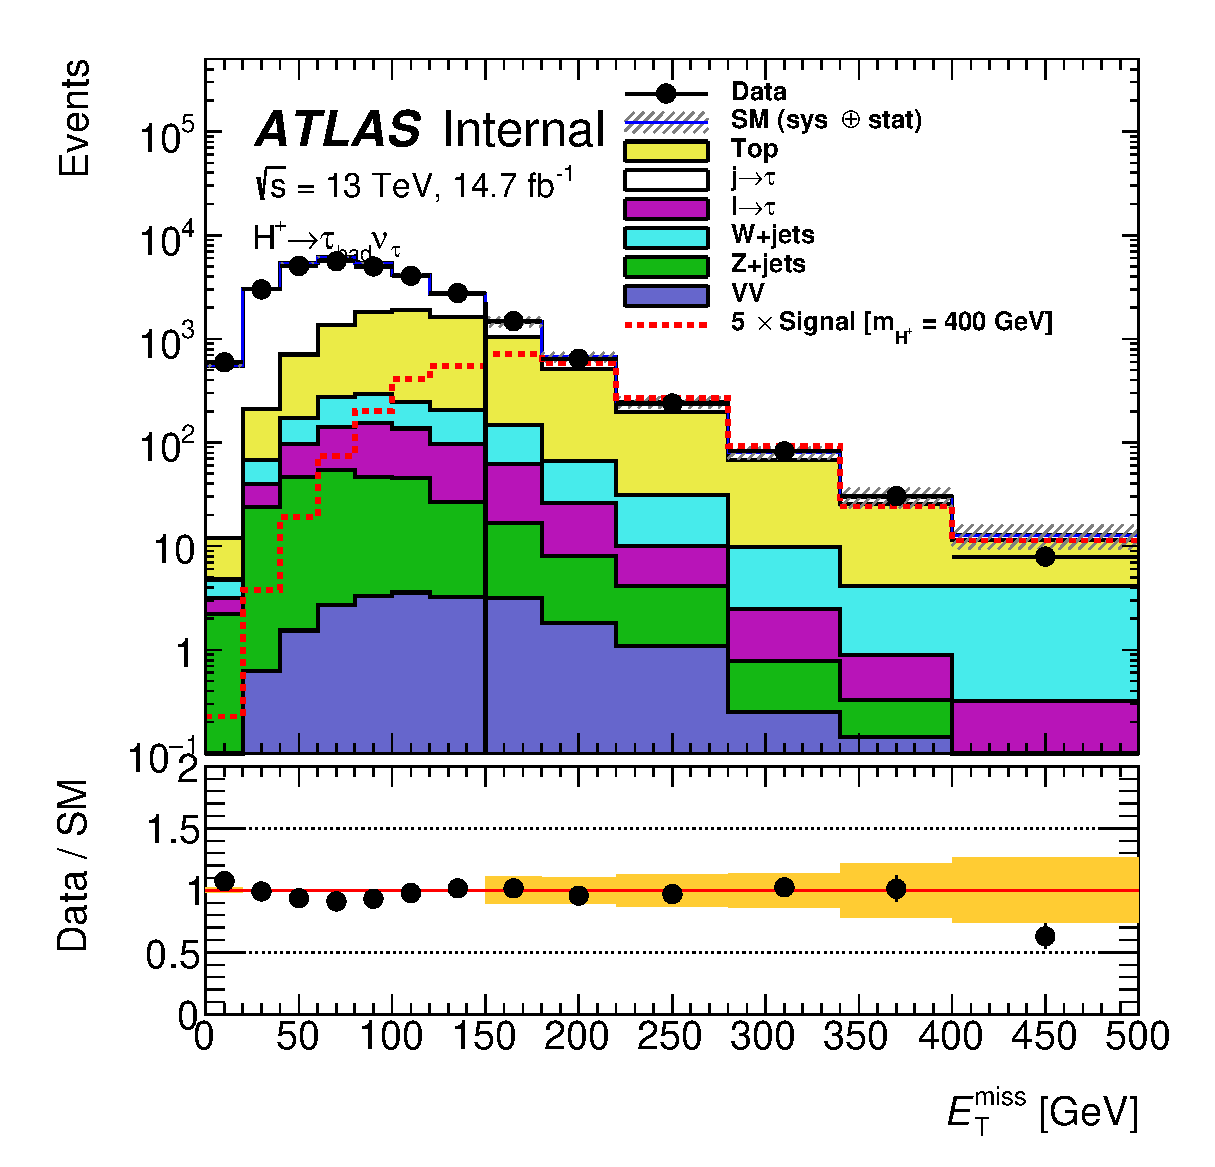
\includegraphics[width=\textwidth]{figures/met_SR_nMinus1.eps}
\caption{\met}
\end{subfigure} % 
\begin{subfigure}{0.5\textwidth}
   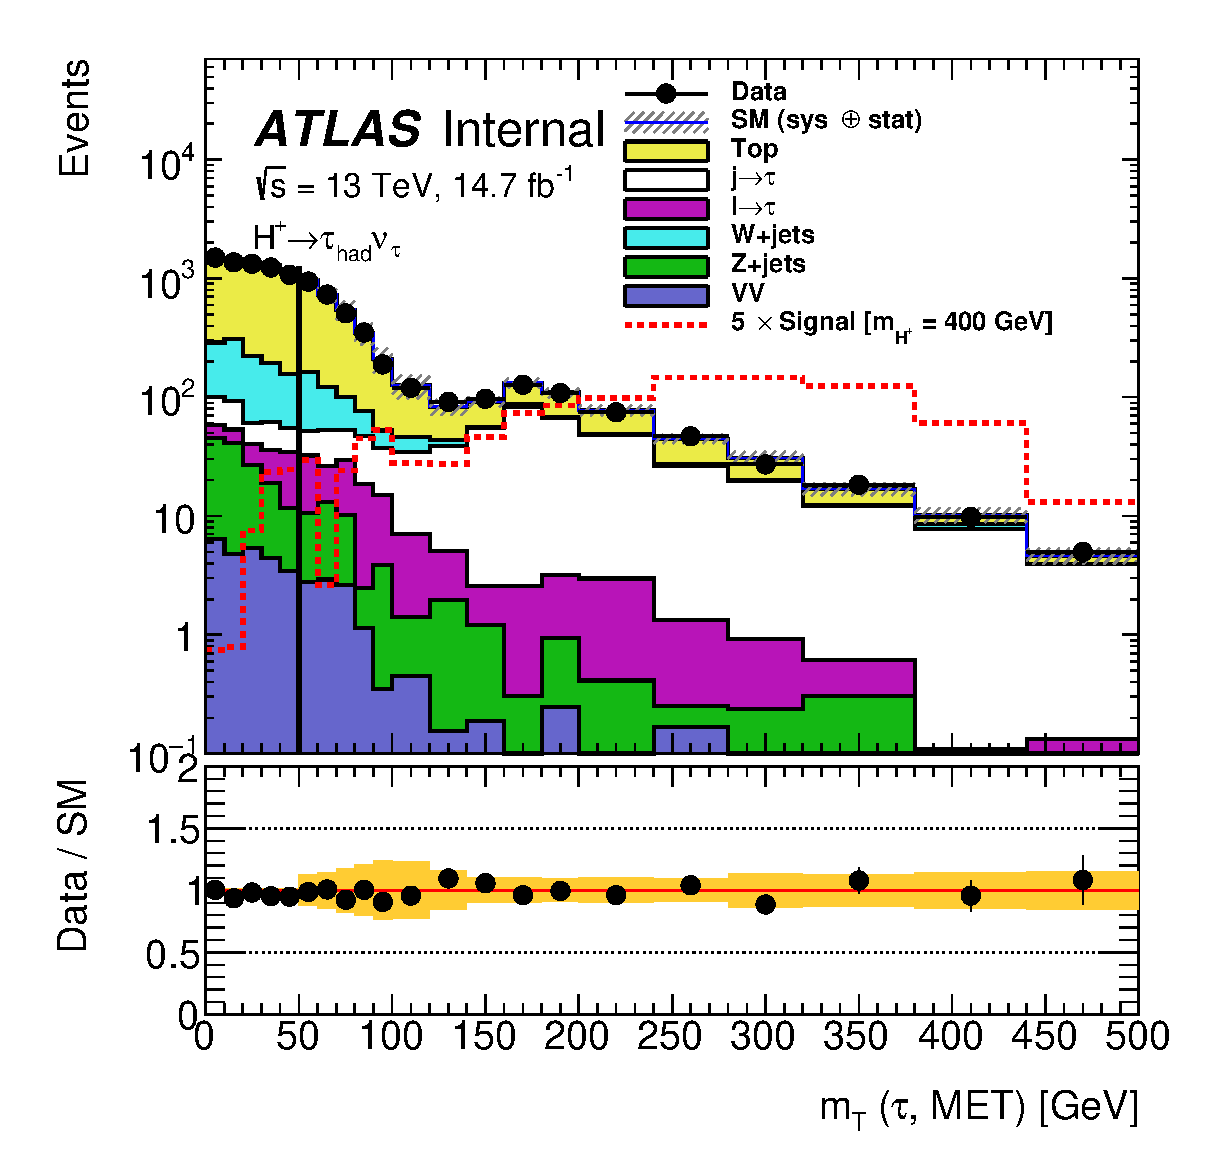
\includegraphics[width=\textwidth]{figures/mT_SR_nMinus1.eps}
\caption{\mT}
\end{subfigure}
\caption{Plots showing the \mT\ and \met\ distributions in the signal region}
\label{fig:primSR}
\end{figure}

\begin{table}[h!]
\centering
\begin{tabular}{|l|r|r|}
\hline
Category & Source & Event Yield \\
\hline\hline
\multirow{4}{*}{True \tauvis} & \ttbar\ + Single Top & 2880$\pm$770$\pm$25 \\
															& $W\to\tau\nu$        & 265$\pm$51$\pm$18   \\
															& $Z\to\tau\tau$       & 44.3$\pm$7.1$\pm$7.6 \\
															& $VV$								 & 13.8$\pm$2.2$\pm$1.7 \\ 
\hline
$j\to\tau$										& All processes				 & 1170$\pm$110$\pm$16 \\
$l\to\tau$										& All processes 			 & 126$\pm$25$\pm$6.5  \\
\hline
	Total Background						&      & 4500$\pm$779$\pm$36.4 \\				
Data (14.7~\ifb)							&											 & 4645   \\
\hline
\end{tabular}
\caption{Expected event yields in the signal region, compared to observed event yields from data.}
\label{tab:yieldsSR}
\end{table}

\par Figures~\ref{fig:secSRa} and~\ref{fig:secSRb} show distributions of other kinematic variables 
in the signal region. These are the $\pt,\eta,\phi$ of the $\tauvis$ , the number of reconstructed jets, the number 
of $b$-tagged reconstructed jets and the $\Delta\phi(\tau,\met)$. All these figures show that the 
\ttbar\ background with true \tauvis\ is the most dominant. 

\begin{figure}[!h]
\begin{subfigure}{0.5\textwidth}
					 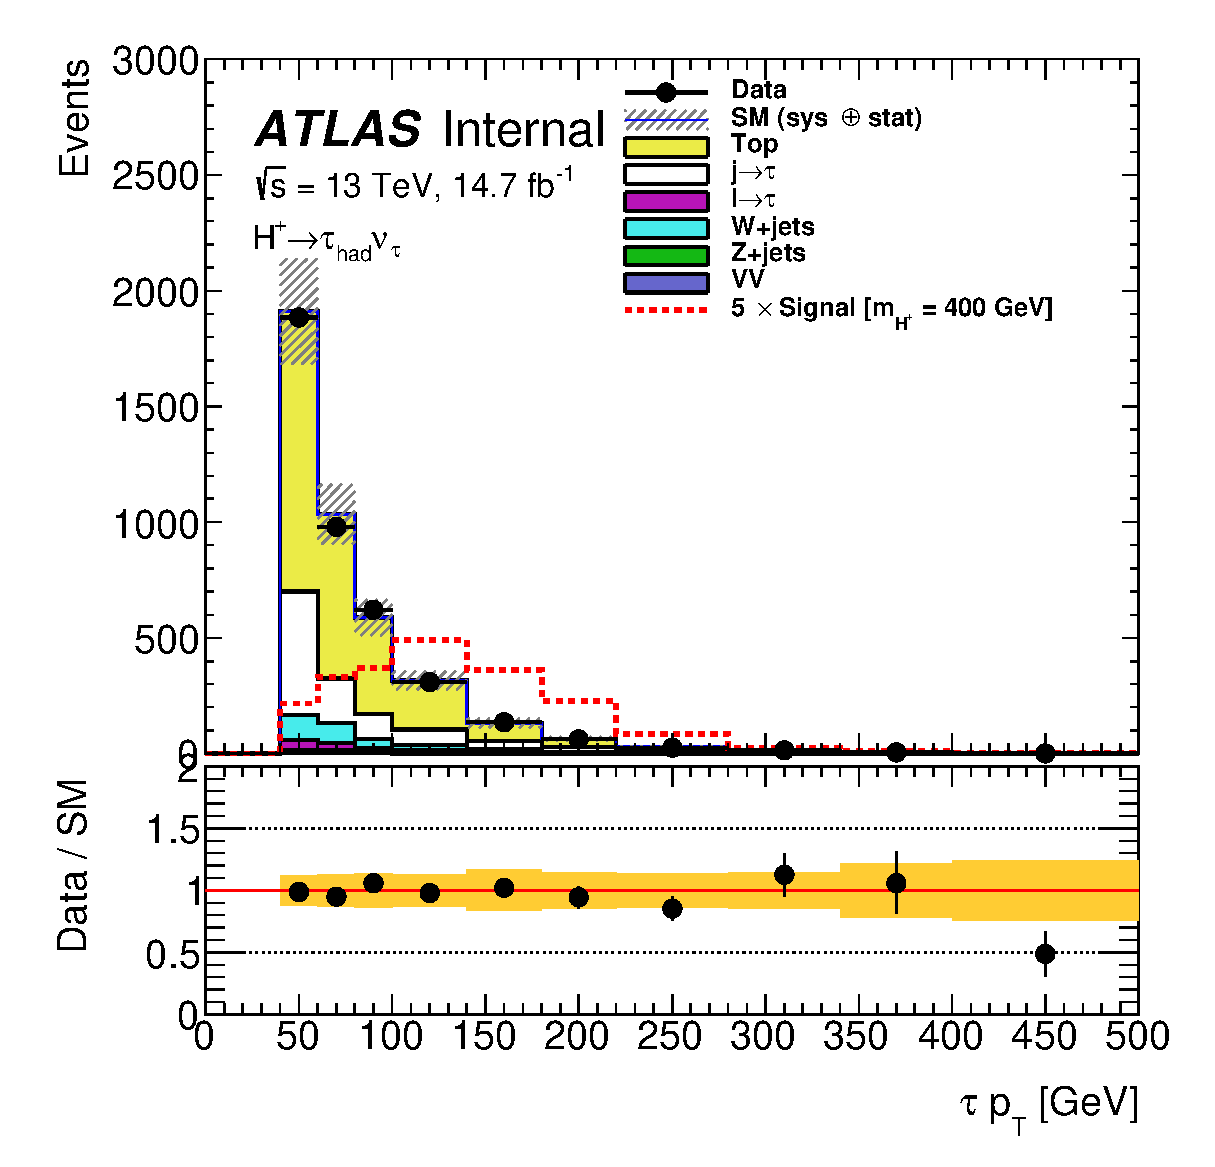
\includegraphics[width=\textwidth]{figures/tauPt_SR.eps}
\end{subfigure}  
\begin{subfigure}{0.5\textwidth}
   \includegraphics[width=\textwidth]{figures/jets_SR.eps}
\end{subfigure}
\begin{subfigure}{0.5\textwidth}
   \includegraphics[width=\textwidth]{figures/bJets_SR.eps}
\end{subfigure} %\\
\begin{subfigure}{0.5\textwidth}
   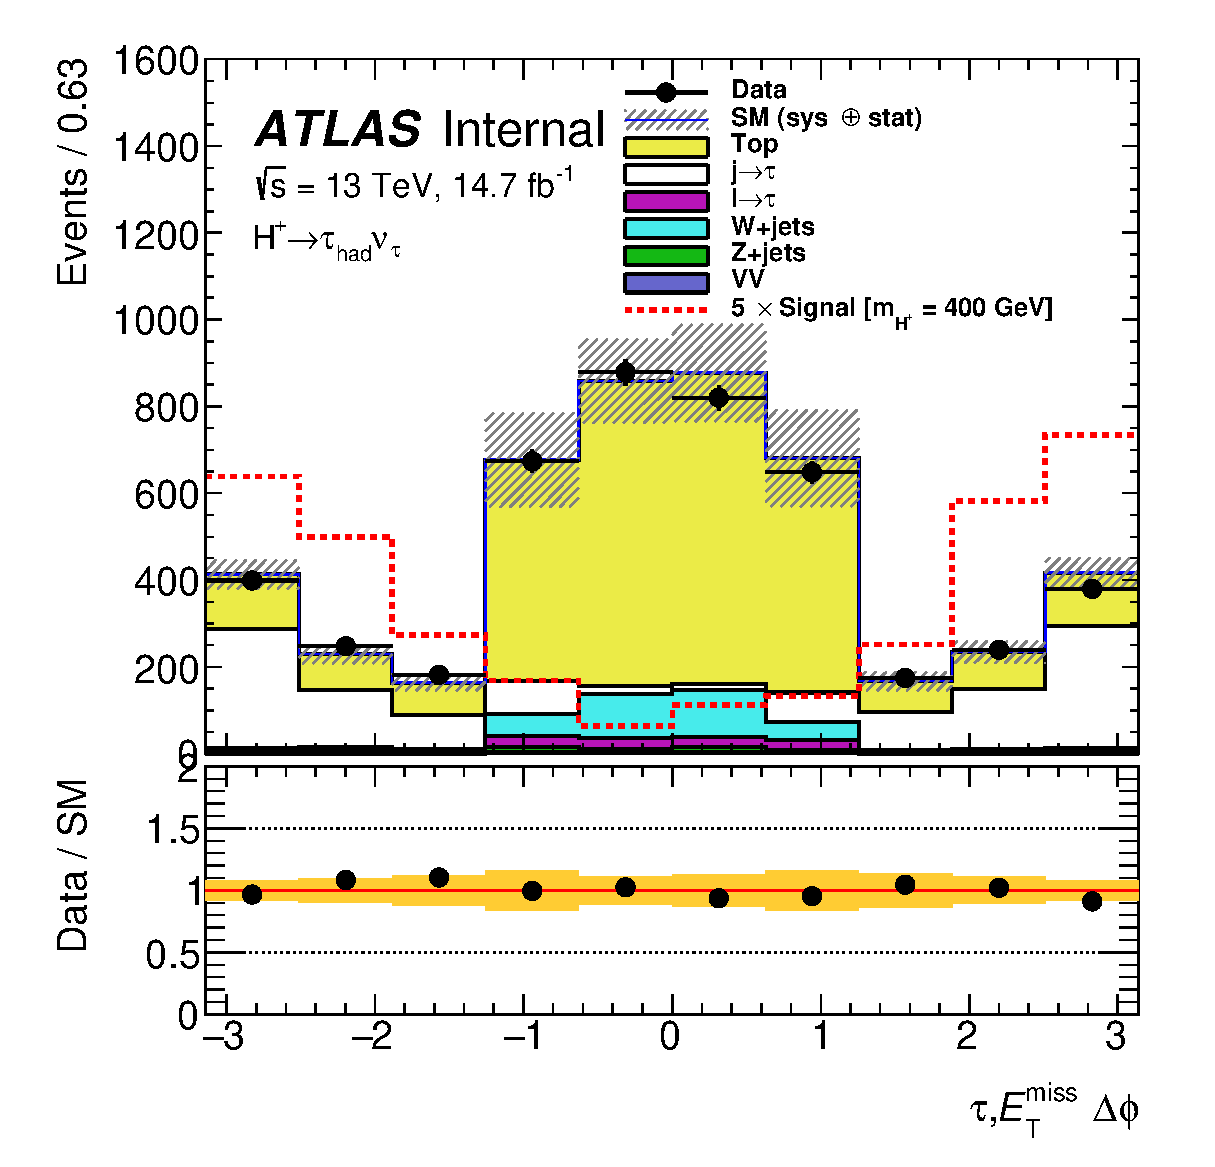
\includegraphics[width=\textwidth]{figures/tauMetPhi_SR.eps}
\end{subfigure}
\caption{Plots showing distributions of \tauvis\ \pt, number of reconstructed 
jets, number of b-tagged jets and the angular separation between the \tauvis\ and \met, 
 in the signal region}
\label{fig:secSRa}
\end{figure}

\begin{figure}[!h]
\begin{subfigure}{0.5\textwidth}
   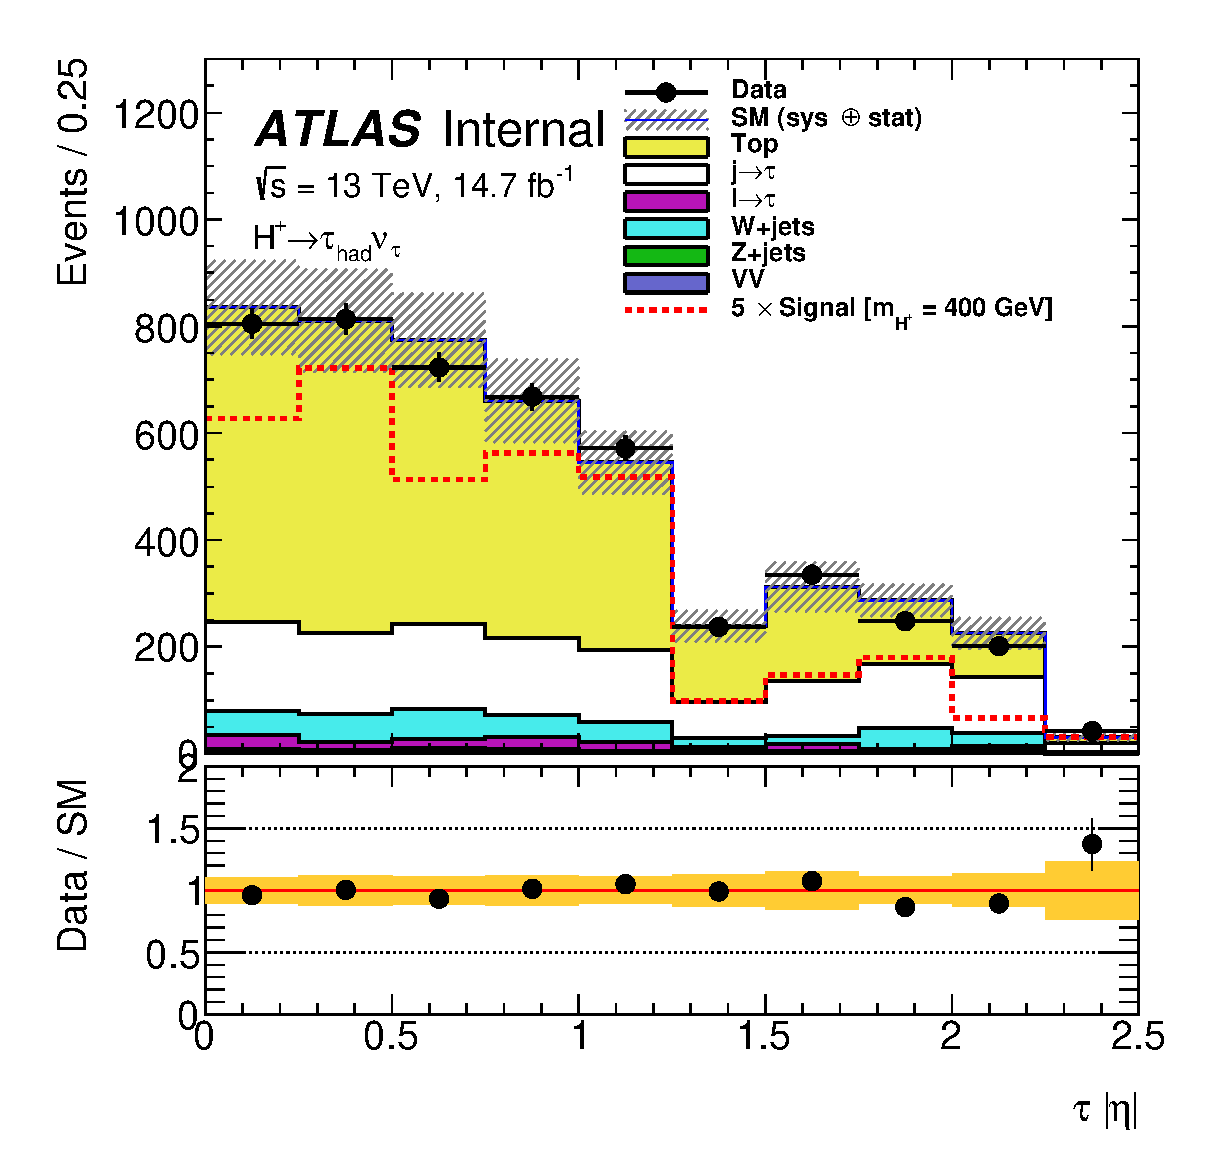
\includegraphics[width=\textwidth]{figures/tauEta_SR.eps}
\end{subfigure}
\begin{subfigure}{0.5\textwidth}
   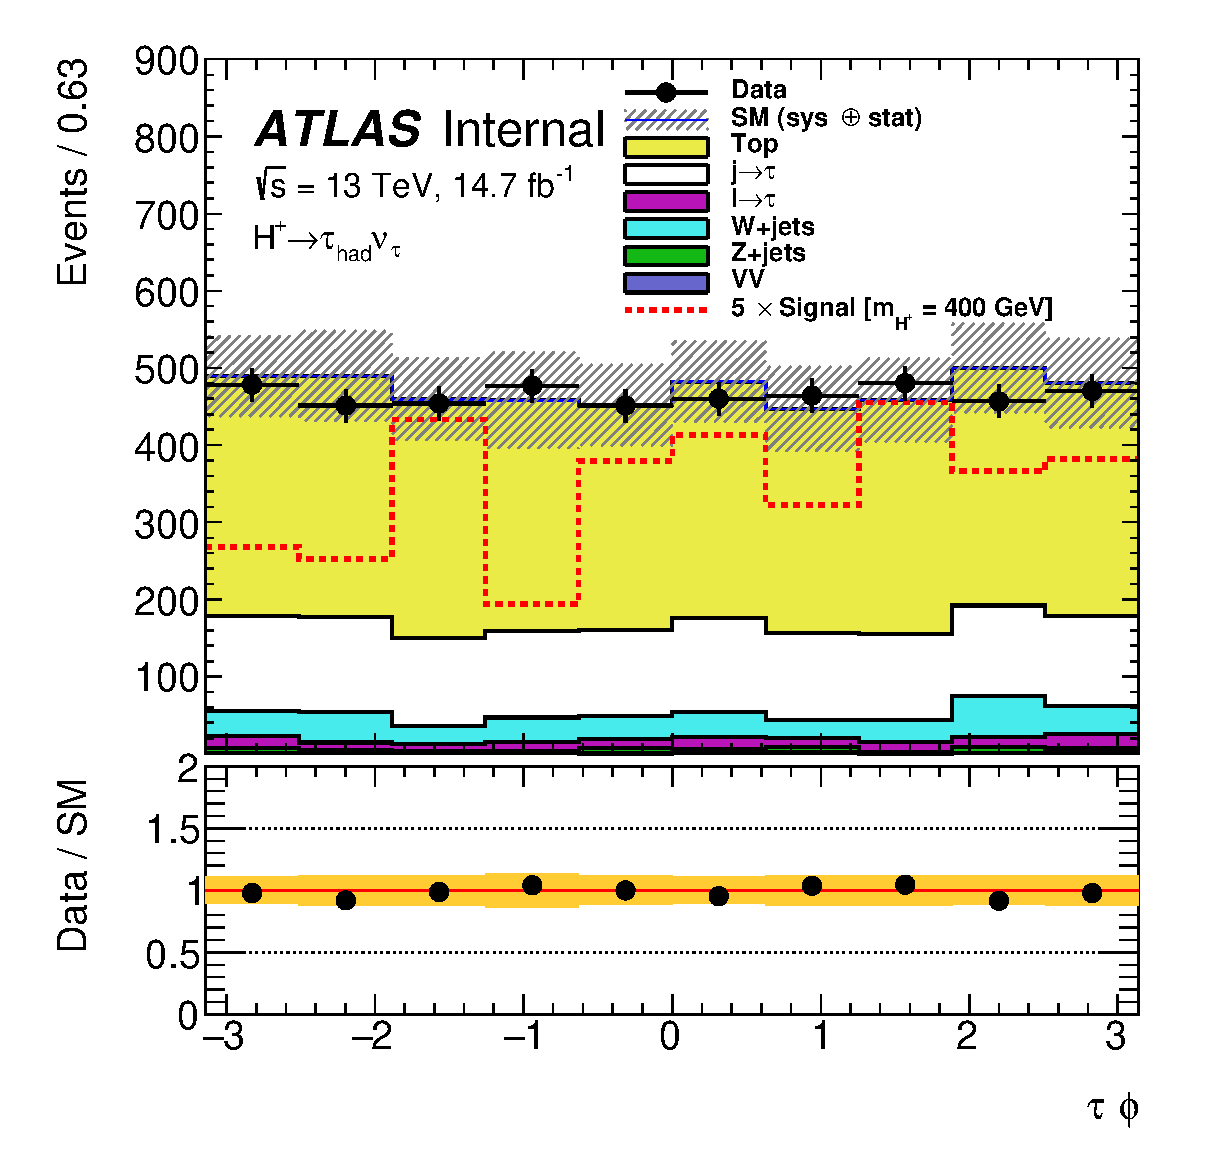
\includegraphics[width=\textwidth]{figures/tauPhi_SR.eps}
\end{subfigure}
\caption{Plots showing distributions of \tauvis\ $\eta$ and $\phi$ in the signal region}
\label{fig:secSRb}
\end{figure}

\subsection{Statistical Analysis}
\label{sec:chStat}
\par Results were tested for evidence of existence of charged Higgs bosons with $\mcH$ ranging 
from 200$\to$2000~\GeV. For each of the mass points, $\sigma^{Exp}_{H^+}$ was set at 
1 to make the parameter of interest $\mu=\sigma^{Obs}_{H^+}$. Here, the said cross section is 
the product of the production cross section and branching ratio of the topologies introduced in 
Equations~\ref{eq:topA} and~\ref{eq:topB}. The test statistic $q_0$, where $\mu=0$ 
in Equation~\ref{eq:testStat}, was used to test the compatibility 
of observed data with the background-only hypothesis. The probability distribution function 
$f(q|b)$ was estimated using the asymptotic approximation~\cite{Cowan:2010js} which 
supposes an artificial data-set called the `Asimov data-set'.\footnote{This data-set is 
defined such that if used to evaluate estimators of all parameters, true values of those 
parameters are obtained}   

\par The systematic uncertainties discussed in 
Section~\ref{sec:systsUnc} were included as nuisance parameters. 
Table~\ref{tab:nuisance_par} shows the list of all such uncertainties and 
the processes (components) to which they were applied. Those that affect more than one 
component were treated as correlated or anti-correlated, whichever was applicable. Otherwise, 
it was assummed that they were uncorrelated. Those whose 
impact on the expected event yield or \mT\ shape is less than 0.5\% were removed from the list.   
The $\pm1\sigma$ variations were symmetrized by taking the one with the largest impact on 
the result, unless there was an explicit reason for an asymmetry.  

\begin{table}[!htb]
 \begin{center}
   \footnotesize
   \begin{tabular}{l p{5cm}|c|ccc}
     {}  &  & signal & true $\tau$ & $j\ra\tau$& $l\ra\tau$ \\
     {}  &  &        & (MC)        & (Data)       & (MC) \\
     \multicolumn{2}{l|}{Contribution to total background (\%)}  &  & 72 &  25 & 3  \\
      \hline \hline            
      NUIP                          & Description &&&&\\
      alpha\_xxx &&&&&\\
      \hline
      JET\_Globally-reduced\_X     & jet energy scale: 19 components       & \ding{51} & \ding{51}  &   \ding{51} &  \ding{51} \\
     JET\_Flavor\_X               & jet energy scale: 3 components  & \ding{51} & \ding{51}  &   \ding{51} &  \ding{51} \\
     JET\_JER\_NP\_X              & jet energy resolution: 8 components  & \ding{51} & \ding{51}  &   \ding{55} &  \ding{51} \\
     TAUS\_TRUEHADTAU\_SME\_TES   & $\tauvis$ energy scale: 3 components    & \ding{51} & \ding{51}  &   \ding{55} & \\
     bjet\_xyz                     & $b$-jet identification SFs: 6 b, 4 c and 10 light components
                                   & \ding{51} & \ding{51} & \ding{51} & \ding{51} \\
     MET\_SoftTrk\_xyz            & $\met$ soft term: 2 resolution, 1 scale component
                                   & \ding{51} &\ding{51} & \ding{55} &\ding{51} \\
     met\_xyz                      & $\met$ trigger efficiency measurement: 3 components
                                   & \ding{51} &\ding{51} & \ding{55} &\ding{51} \\
     signal\_xyz                   & theoretical uncertainty on signal acceptance: QCD scale and PSUE
                                   & \ding{51} & & & \\
     ttbar\_xzy                    & theoretical uncertainty on \ttbar~acceptance and \mT~shape: scale, PSUE, ME    
                                   & &\ding{51} & &\\
     ttbar\_norm                   & \ttbar~cross section
                                   & &\ding{51} & &\\
     UWSF                          & $W\ra\tau\nu$ scale factor uncertainty
                                   & &\ding{51} & &\\
     lep\_sf                       & $\ell\rightarrow\tauvis$ scale factor  
                                   & & & & \ding{51} \\
     tau\_ID                       & $\tauvis$ identification: 2 components (all and high \pt)
                                   & \ding{51} & \ding{51} & \ding{51} & \\
     tau\_RECO                     & $\tauvis$ reconstruction efficiency
                                   & \ding{51} & \ding{51} & \ding{51} & \\
     tau\_ELEOLR                   & $\tauvis$/electron overlap removal        & \ding{51} & \ding{51} & \ding{51} & \\
     tau\_ff\_stat                 & statistics in FF method                      &  &  & \ding{51} & \\
     tau\_ff\_bdt                 & jet composition in FF method                 &  &  & \ding{51} & \\
     tau\_ff\_prompt\_tau          & mis-id prompt $\tauvis$ modelling in MC            &  &  & \ding{51} & \\
   \end{tabular}
 \end{center}
 \caption{
   Description of each of the nuisance parameters, along with
   the samples they were applied to.  If the same nuisance parameter
   was applied to different backgrounds, all correlations were kept. 
 A '\ding{51}' indicates that the systematic uncertainty was considered and included in the fit. A
   '\ding{55}' indicates that the systematic uncertainty was considered but not included in the fit, otherwise
   the given systematic uncertainty is not applied to the given background.}
\label{tab:nuisance_par}
\end{table}

\par The test of the observed data against the background-only hypothesis shows that the data 
is consistent with the Standard Model prediction. Hence, exclusion limits on  
$\mu=\sigma^{Obs}_{H^+}$ were set by rejecting the $s+b$ hypothesis at 95\% confidence 
level using the $CL_s$ procedure, where $CL_s(\mu)$ is defined as in Equation~\ref{eq:cls}.
Expected exclusion limits were computed assuming the $s+b$ hypothesis, and using the artificial 
Asimov data-set which was approximated by the sum of all the expected backgrounds. Observed 
exclusion limits are computed using the $s+b$ hypothesis, and using the total observed 
data. Figures~\ref{fig:exclLimA} and~\ref{fig:exclLimB} show the expected and observed exclusion limits for \mcH\ ranging 
from 200$\to$2000~\GeV. In the former figure, systematic uncertainties were not included in the computation 
of the exclusion limits. In the latter, the systematic uncertainties were included. 
The solid line denotes the observed limits and the dashed line denotes 
the expected limits at 95\% confidence levels. The green and yellow shaded regions represent the 
$\pm1\sigma$ and $\pm2\sigma$ uncertainty bands respectively. An illustrative signal prediction in 
the hMSSM benchmark scenario at $\tan\beta=60$ is also overlayed. Without systematic 
uncertainties the limits are slightly more stringent than with systematic uncertainties.	 
Figure~\ref{fig:exclLimB} shows that the \mcH\ range from 200$\to$540~\GeV for 
$\tan\beta=60$ is excluded by these observed exclusion limits. 

\begin{figure}[!h]
\centering
					 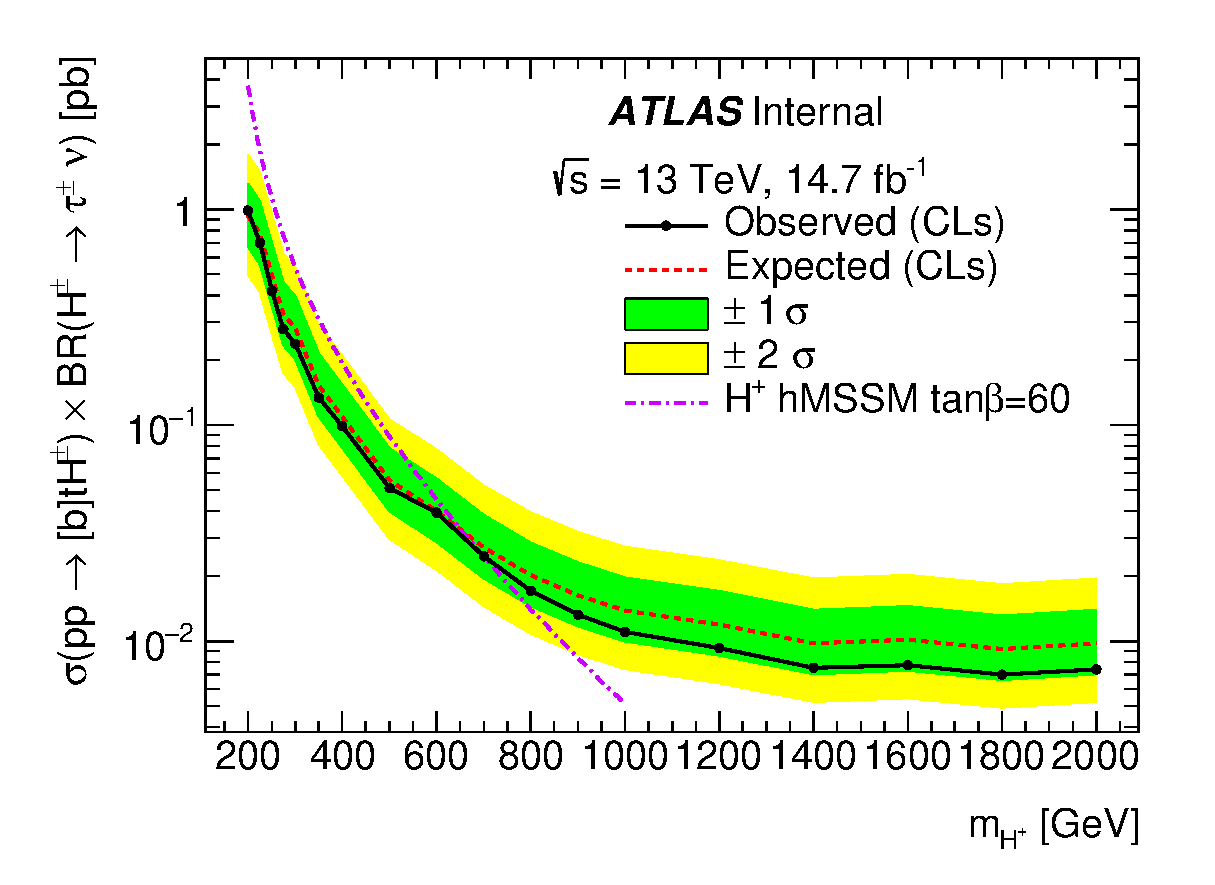
\includegraphics[width=0.8\textwidth]{figures/final_limits_no_sys_asym_limit_log.eps}
\caption{Plots of the expected and observed limits on $\mu=\sigma^{Obs}_{H^+}$, without including systematic uncertainties in the 
background and signal predictions}
\label{fig:exclLimA}
\end{figure}  

\begin{figure}[!h]
\centering
					 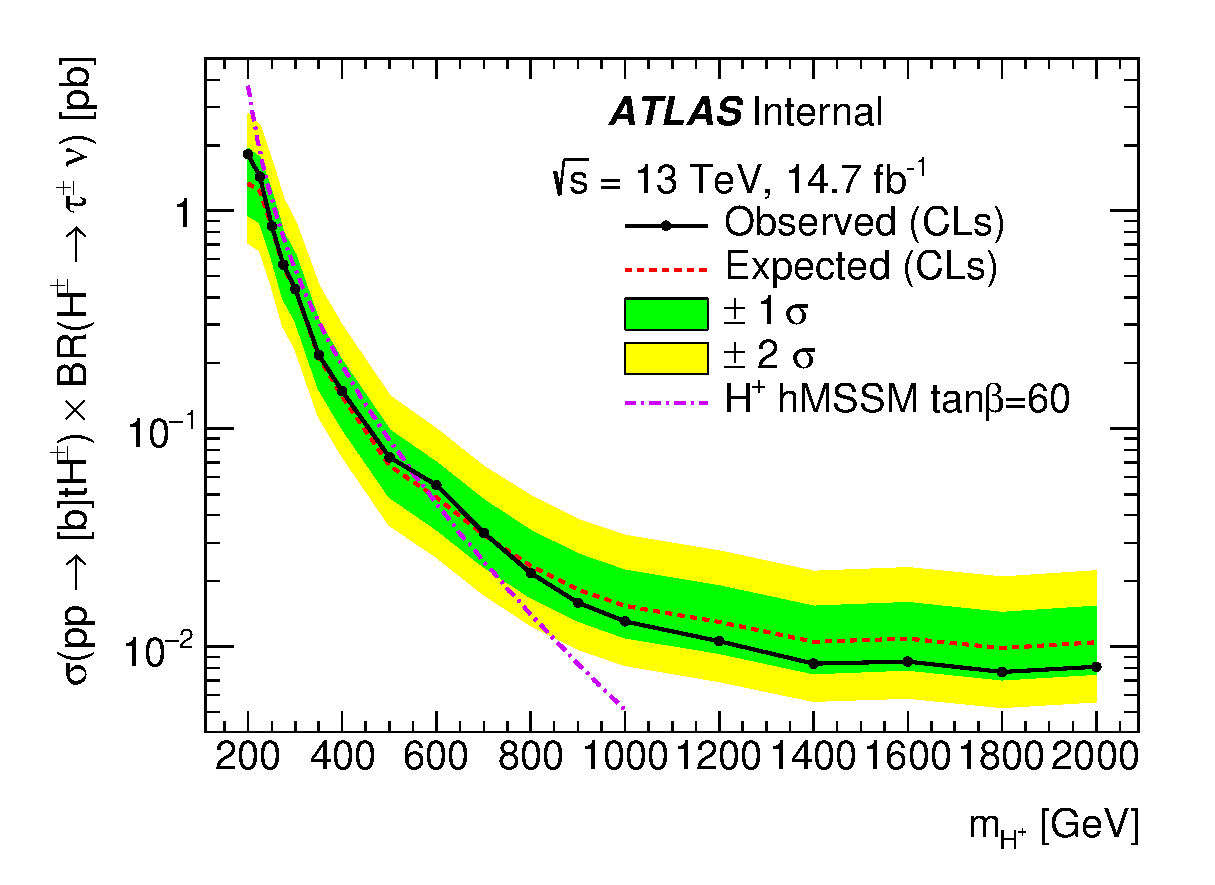
\includegraphics[width=0.8\textwidth]{figures/final_limits_sys_asym_limit_log.eps}
\caption{Plots of the expected and observed limits on $\mu=\sigma^{Obs}_{H^+}$. Systematic uncertainties were included  
in the background and signal predictions}
\label{fig:exclLimB}
\end{figure}

\par To evaluate the impact of the individual limits on exclusion limits shown in Figure~\ref{fig:exclLimB} 
the limit-setting procedure was repeatedly performed without including each of the systematic 
uncertainties. Table~\ref{tab:syst_taujets_postfit} summarizes the impacts of groups of these 
systematic uncertainties for $\mcH=200~\GeV$ and $\mcH=1~\TeV$. The percentage impact was obtained 
by comparing the nominal expected limit and the expected limit computed without considering each of 
these groups of uncertainties. Evidently, the largest impact is from fake factos and \ttbar\ background 
modelling.    

\begin{table}[h!]
 \begin{center}
  \resizebox{\textwidth}{!}{
   \begin{tabular}{|l|l|cc|}
\hline
Category    &  Source of systematic & \multicolumn{2}{c|}{Impact on the expected limit (in \%)} \\
    &  uncertainty & $m_{H^+} = 200~\GeV$ & $m_{H^+} = 1000~\GeV$ \\
     \hline\hline
	\multirow{5}{*}{Experimental} & luminosity  &  $\phantom{0}1.5$   &  $\phantom{0}0.9$ \\
     & trigger  &  $<0.1$  &  $<0.1$ \\
     & $\tau_{\text{had-vis}}$  &  $\phantom{0}1.0$   &  $\phantom{0}1.4$ \\
     & jet  &  $\phantom{0}3.0$   &  $\phantom{0}0.2$ \\
     & $\met$  &  $<0.1$   &  $<0.1$ \\
     \hline
 \multirow{1}{*}{Fake factors} &  \FF  &  $\phantom{0}0.8$   &  $\phantom{0}4.7$ \\
     \hline
 \multirow{2}{*}{Signal and background models}    & $t\bar{t}$ modelling   &  $\phantom{0}13.2$   &  $\phantom{0}3.5$ \\
     & $H^+$ signal modelling  &  $\phantom{0}1.4$   &  $\phantom{0}1.4$ \\
     \hline
   \end{tabular}
}
   \caption{Impact of various sources of uncertainty on
      the expected 95\% CL exclusion limit.}
\label{tab:syst_taujets_postfit}
  \end{center}
\end{table}

